\section{Trapezoidal rule}
\label{sec:trapezoid}

In this exercise, you are tasked with implementing the simple trapezoid
rule formula for numerical integration. If we want to compute the
definite integral \begin{equation}
\int_{a}^{b}f(x)dx\end{equation}
we can partition the integration interval $[a,b]$ into smaller subintervals,
and approximate the area under the curve for each subinterval by the
area of the trapezoid created by linearly interpolating between the
two function values at each end of the subinterval. This is graphically
illustrated in Figure~\ref{fig:trapezoid}, where the blue line represents
the function $f(x)$ and the red line represents the successive linear
segments.

The area under $f(x)$ (the value of the definite integral) can thus
be approximated as the sum of the areas of all these trapezoids. If
we denote by $x_{i}$ ($i=0,\ldots,n,$ with $x_{0}=a$ and $x_{n}=b$)
the abscissas where the function is sampled, then \begin{equation}
\int_{a}^{b}f(x)dx\approx\frac{1}{2}\sum_{i=1}^{n}\left(x_{i}-x_{i-1}\right)\left(f(x_{i})+f(x_{i+1})\right).\label{eq:trapzf}\end{equation}
The common case of using equally spaced abscissas with spacing $h=(b-a)/n$
reads simply \begin{equation}
\int_{a}^{b}f(x)dx\approx\frac{h}{2}\sum_{i=1}^{n}\left(f(x_{i})+f(x_{i+1})\right).\label{eq:trapzf2}\end{equation}
One frequently receives the function values already precomputed, $y_{i}=f(x_{i}),$
so equation~(\ref{eq:trapzf}) becomes \begin{equation}
\int_{a}^{b}f(x)dx\approx\frac{1}{2}\sum_{i=1}^{n}\left(x_{i}-x_{i-1}\right)\left(y_{i}+y_{i-1}\right).\label{eq:trapz}\end{equation}


%
\begin{figure}
\begin{centering}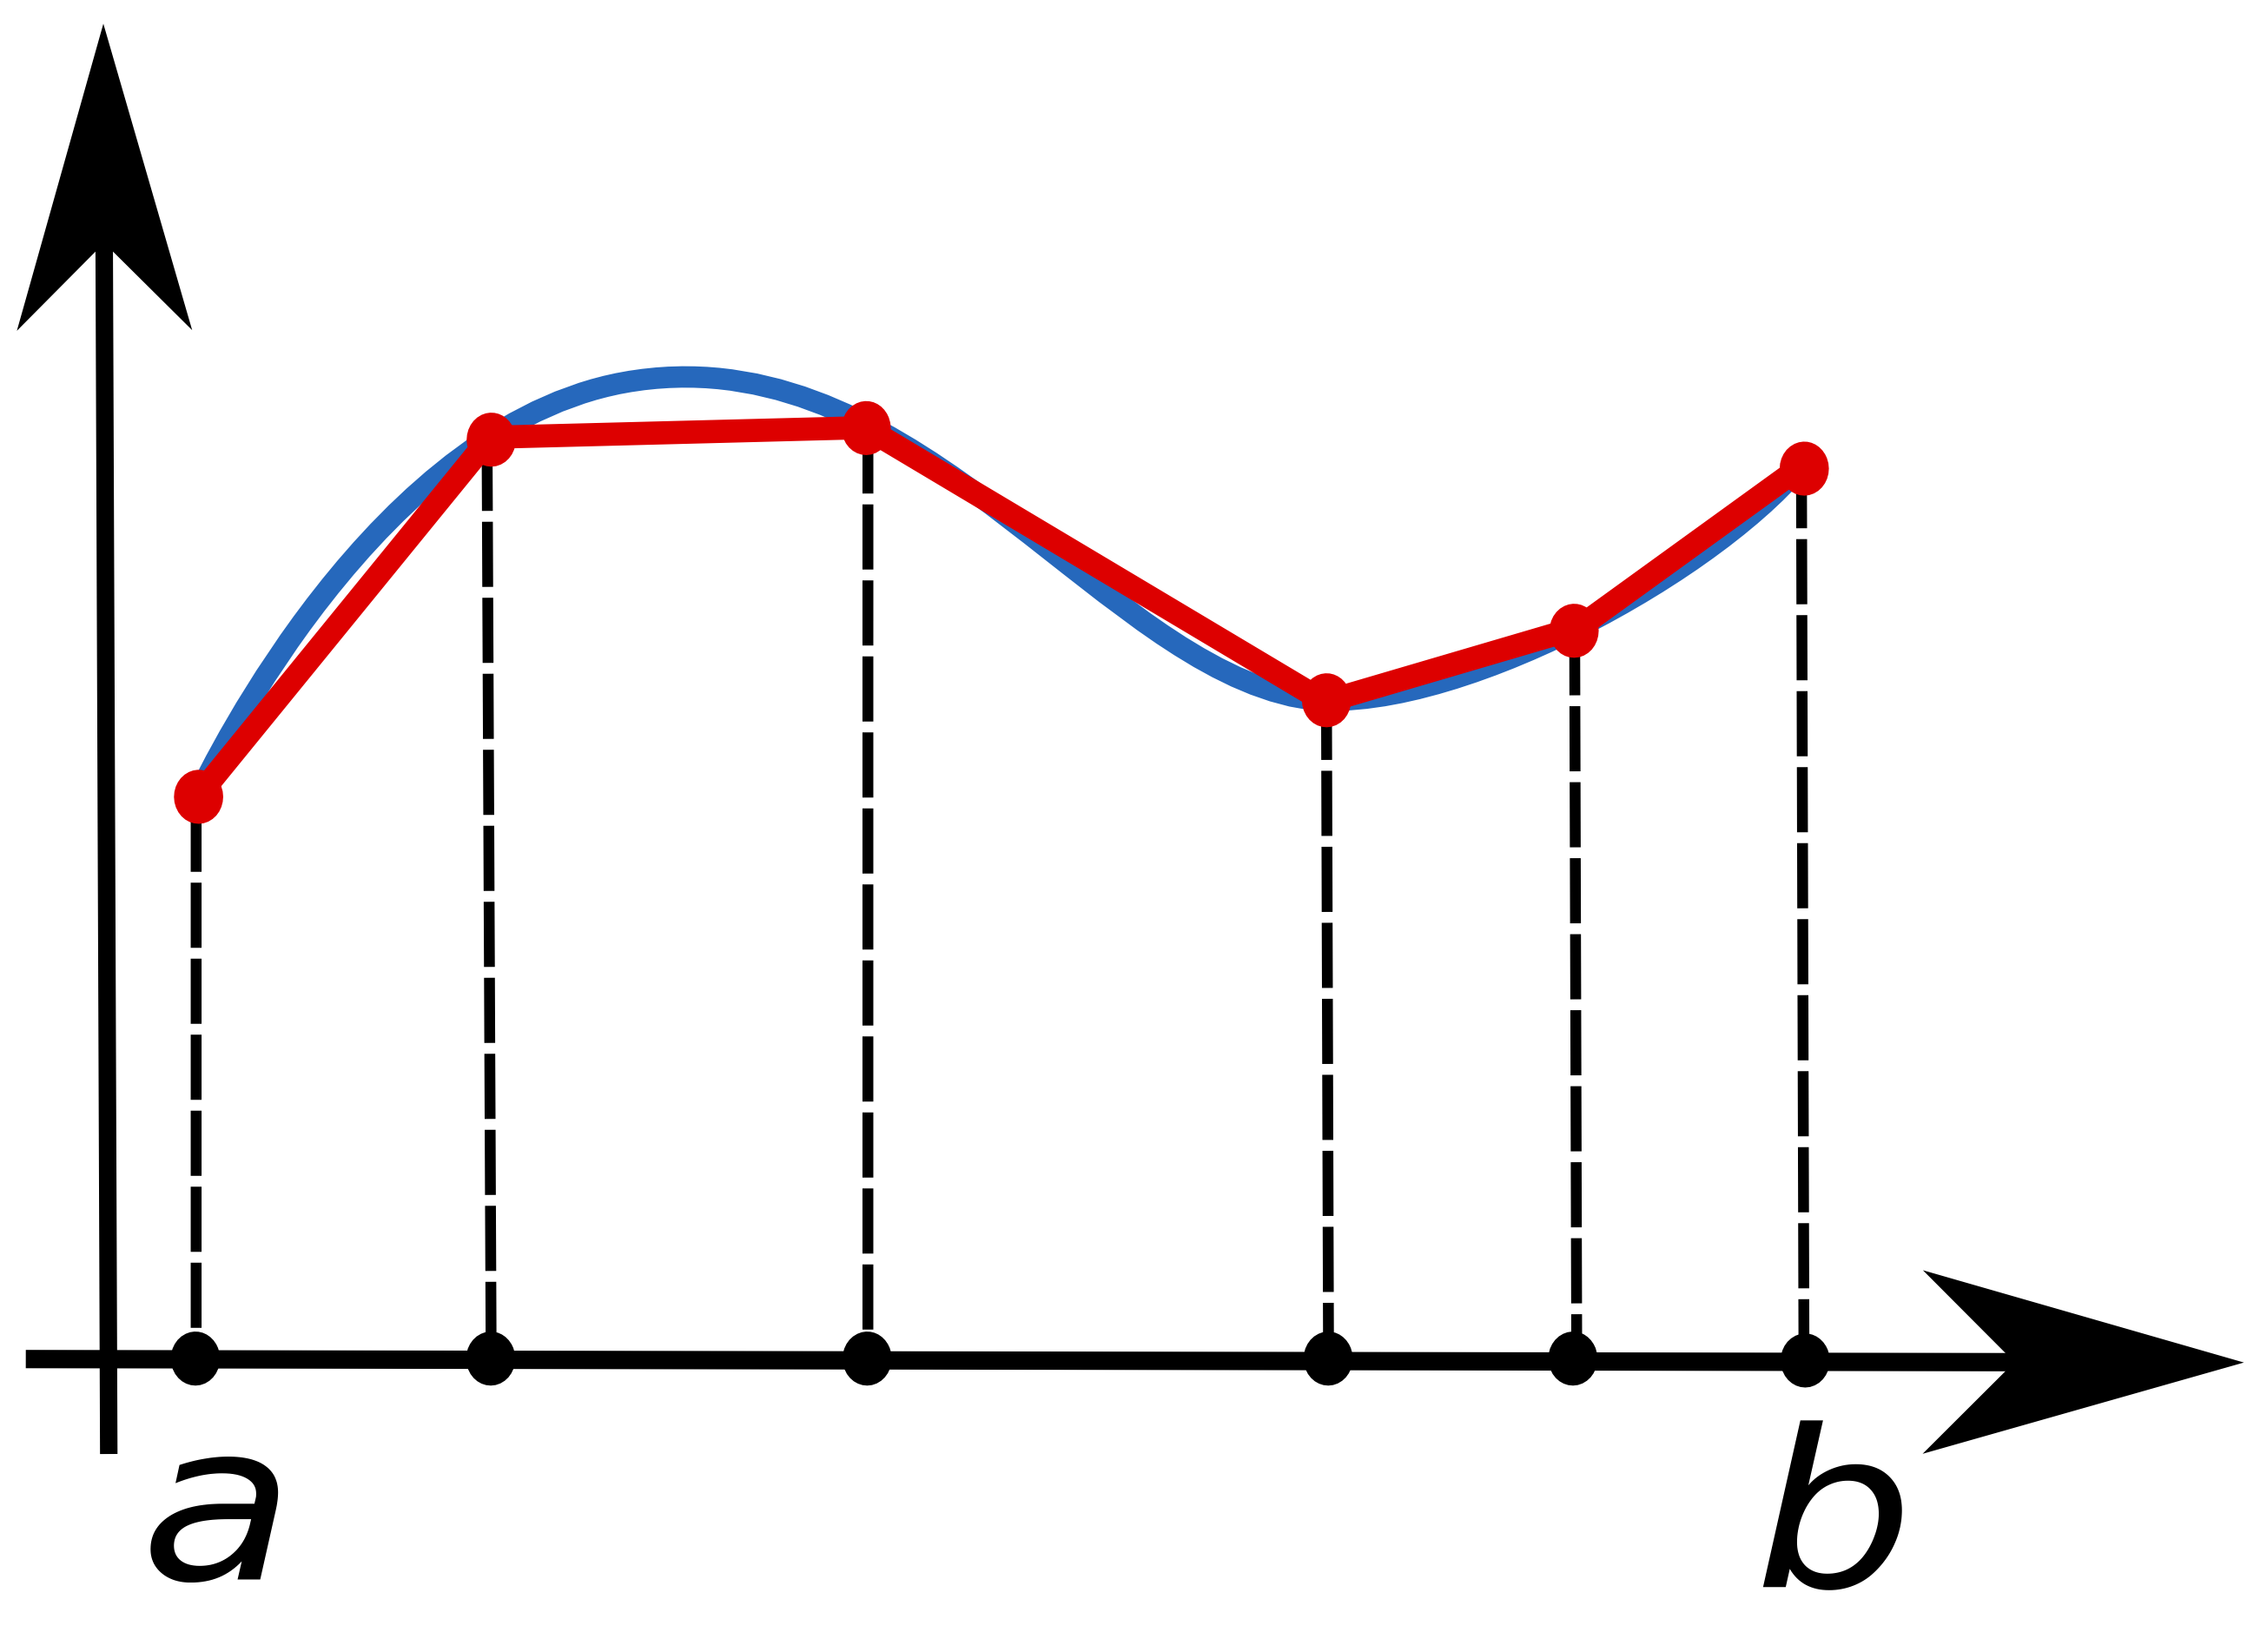
\includegraphics[width=4in]{fig/Composite_trapezoidal_rule_illustration}\par\end{centering}


\caption{\label{fig:trapezoid}Illustration of the composite trapezoidal rule
with a non-uniform grid (Image credit: Wikipedia).}
\end{figure}


Listing~\ref{code:trapezoid} contains a skeleton for this problem,
written in the form of two incomplete functions and a set of automatic
tests (in the form of \emph{unit tests}, as described in the introduction).

\lstinputlisting[label=code:trapezoid,caption={IGNORED}]{problems/trapezoid.py}

In this exercise, you'll need to write two functions, \texttt{trapz}
and \texttt{trapzf}. \texttt{trapz} applies the trapezoid formula
to pre-computed values, implementing equation~(\ref{eq:trapz}),
while \texttt{trapzf} takes a function $f$ as input, as well as the
total number of samples to evaluate, and computes eq.~(\ref{eq:trapzf2}).
